\chapter{Introduction}

\section{Overview}

Antimicrobial resistance (AMR) represents one of the most pressing global health challenges of the 21st century. The World Health Organization has identified AMR as a top-ten global public health threat, with projections estimating that bacterial infections could result in approximately 10 million deaths annually by 2050 if current trends continue \cite{oneill2016amr}. In 2019 alone, antibiotic-resistant bacteria directly caused 1.27 million deaths, with an additional 4.95 million deaths associated with drug-resistant infections \cite{amr2019lancet}. Critical priority pathogens including \textit{Klebsiella pneumoniae}, \textit{Escherichia coli}, \textit{Pseudomonas aeruginosa}, and \textit{Salmonella enterica} account for a substantial proportion of these deaths, with carbapenem-resistant strains posing particular clinical challenges.

Traditional culture-based antimicrobial susceptibility testing (AST) remains the gold standard for determining resistance profiles but suffers from significant limitations. Most culturable bacteria require 24--48 hours of incubation for detection, with pathogen identification adding another 2--4 hours. If AMR is suspected, phenotypic AST extends the timeline by an additional 18--24 hours, resulting in a total turnaround time of 2--4 days \cite{ahmad2023ast}. This delay can prove critical in severe infections where rapid administration of appropriate antimicrobials significantly improves patient outcomes---the risk of death doubles if effective antibiotics are not administered within 24 hours in cases of bacteremia \cite{kumar2006sepsis}.

The advent of whole genome sequencing (WGS) and the establishment of comprehensive resistance gene databases have enabled computational approaches to AMR prediction. Machine learning (ML) methods have emerged as powerful tools for predicting resistance phenotypes from genomic data, offering the potential for rapid, accurate predictions that could guide empirical therapy selection before traditional AST results become available \cite{maguire2022ml}. This thesis presents a resistance gene-based machine learning framework that addresses critical methodological gaps in current AMR prediction approaches, demonstrating that optimized gene-based models can achieve performance competitive with or superior to whole-genome sequence-based methods while maintaining interpretability and computational efficiency.

Figure~\ref{fig:amr_framework} illustrates the difference between traditional culture-based prediction and modern ML-based genomic prediction.

\begin{figure}[h]
\centering
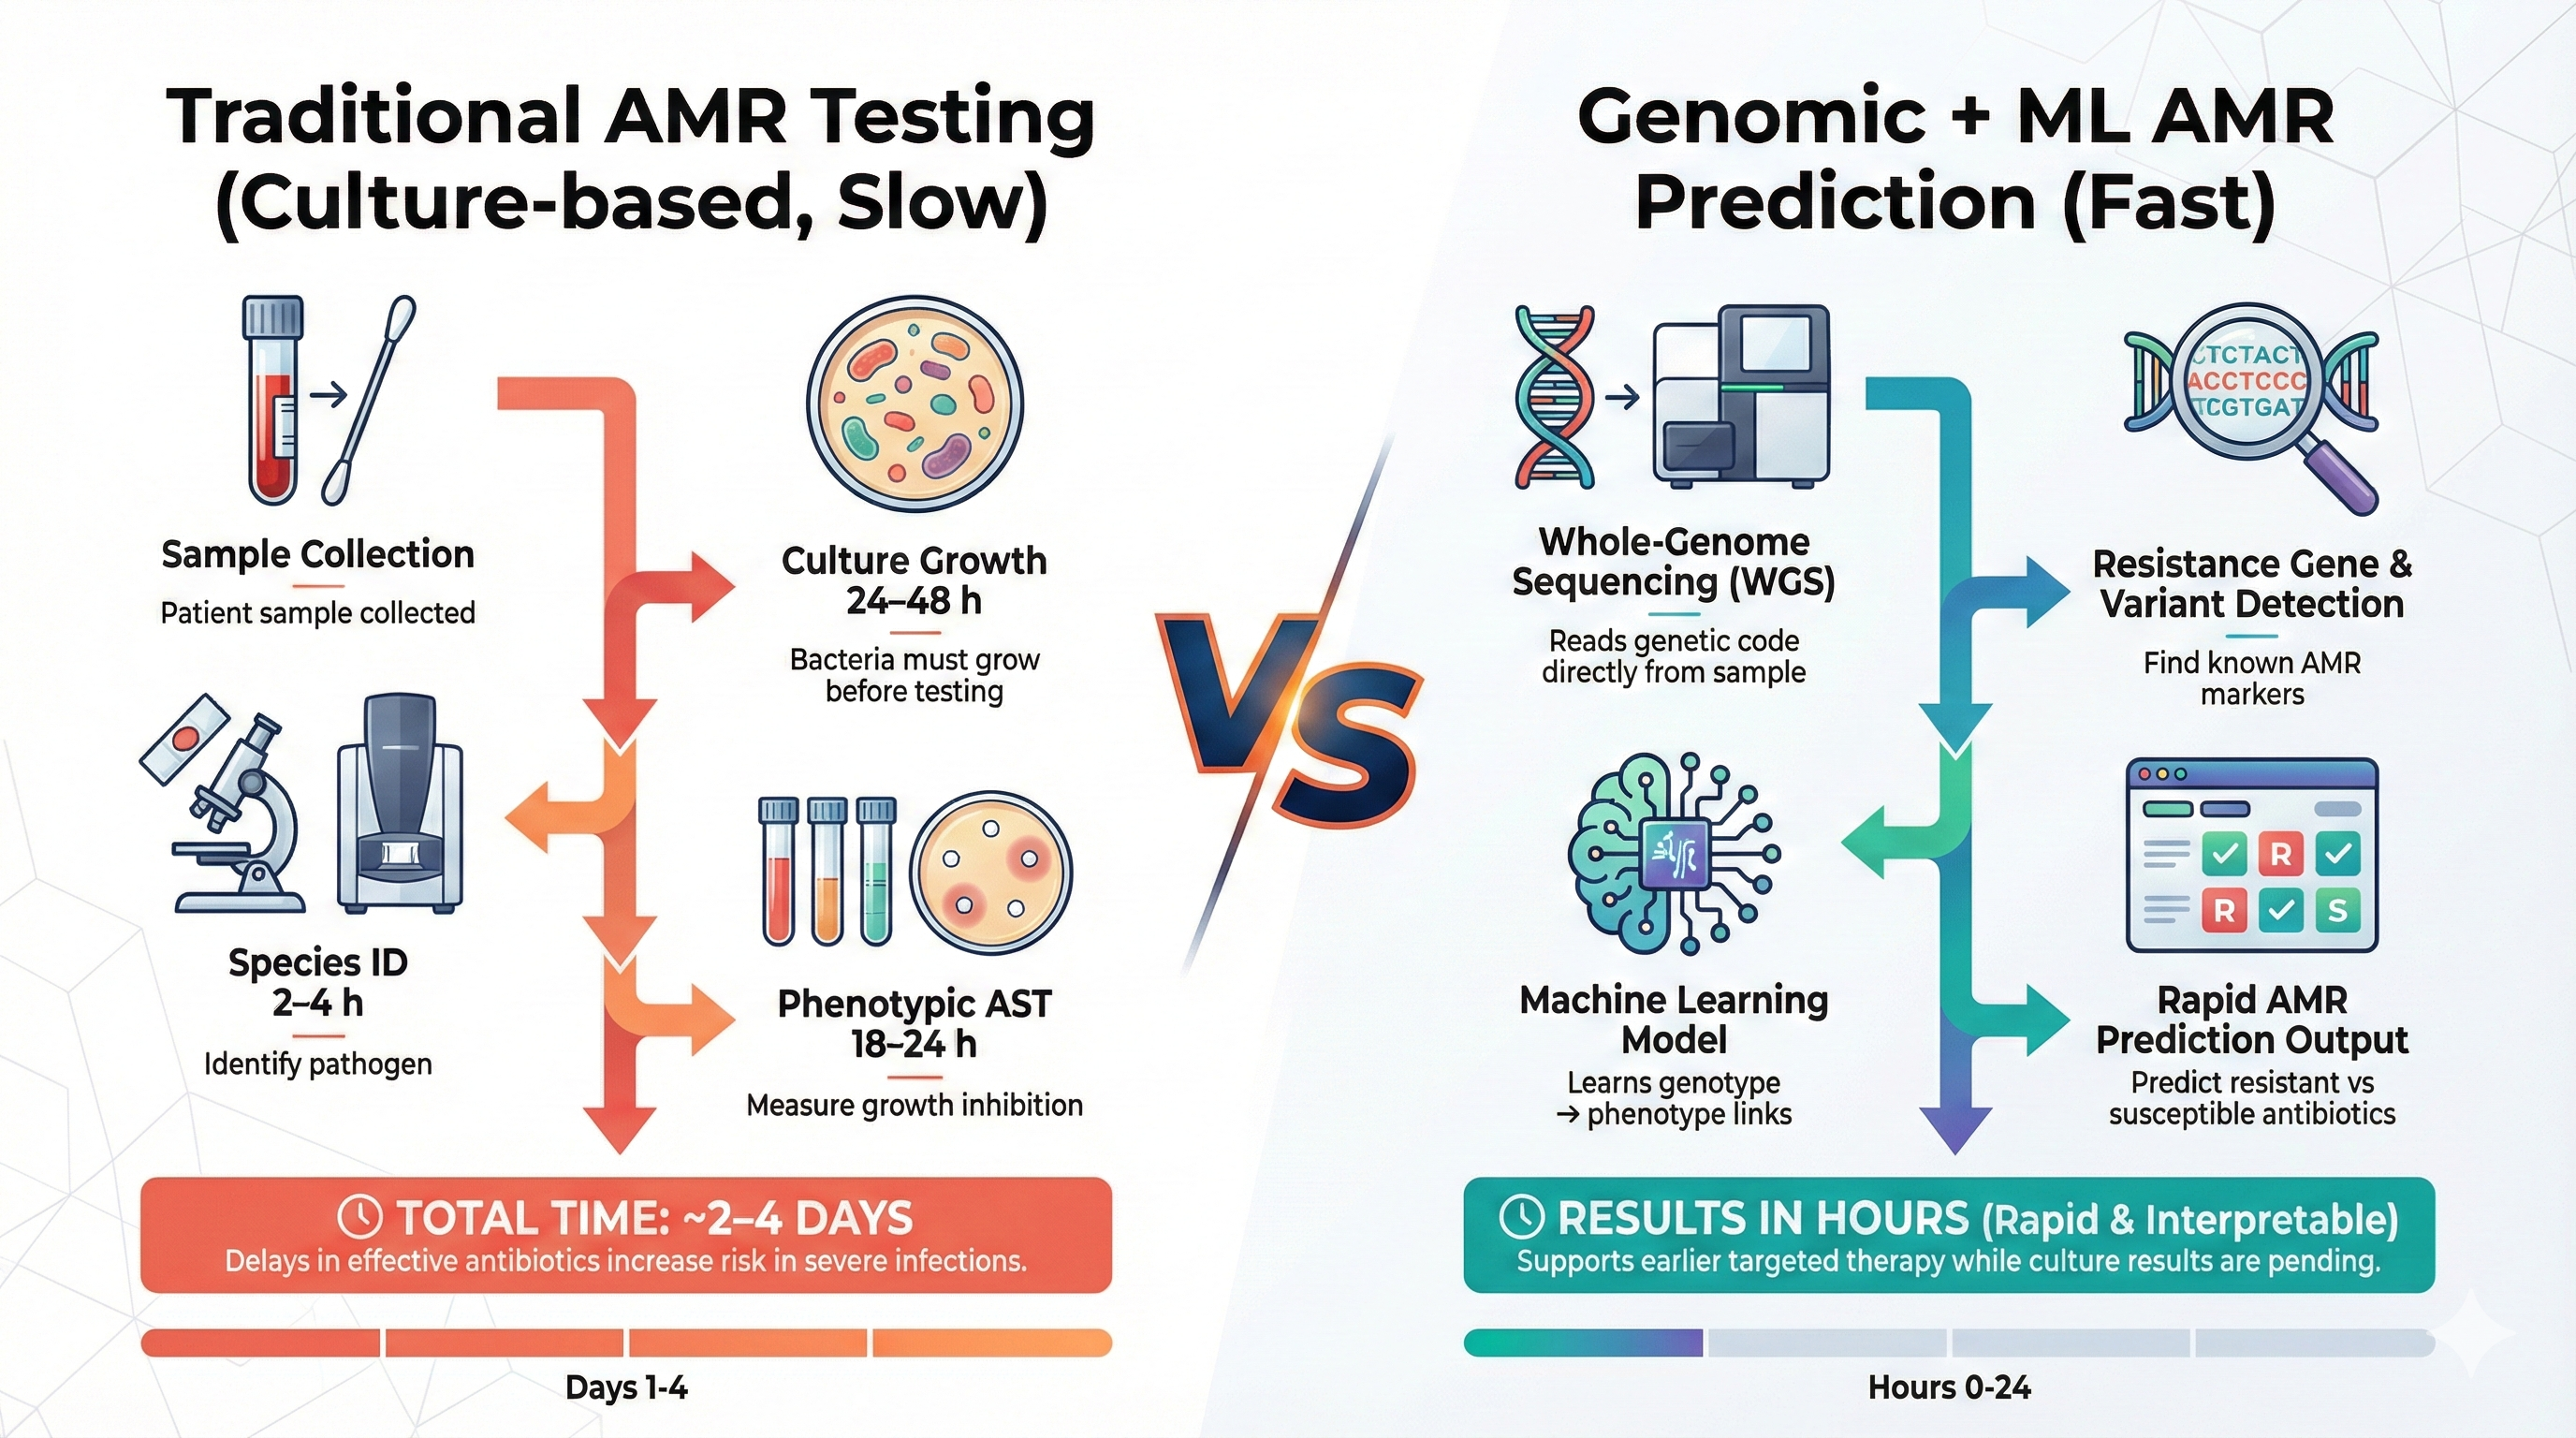
\includegraphics[width=0.8\textwidth]{figures/Traditional vs genomic.png}
\caption{Traditional AMR testing vs genomic + ML AMR prediction}
\label{fig:amr_framework}
\end{figure}


\section{Antimicrobial Resistance: A Global Health Crisis}

Antimicrobial resistance occurs when bacteria, viruses, fungi, and parasites evolve mechanisms to survive exposure to antimicrobial drugs that previously killed them or inhibited their growth. For bacteria, resistance mechanisms include enzymatic degradation (e.g., $\beta$-lactamases hydrolyzing penicillins and cephalosporins), modification of drug targets (e.g., mutations in DNA gyrase conferring fluoroquinolone resistance), efflux pump overexpression, and reduced membrane permeability \cite{murray2022harrison}.

Resistant infections lead to longer hospital stays, higher medical costs, and increased mortality. Patients with drug-resistant infections face a 64\% higher risk of death compared to those with susceptible infections \cite{klein2018antibiotic}. Beyond individual outcomes, AMR threatens the effectiveness of organ transplantation, cancer chemotherapy, and complex surgeries that rely on antimicrobial prophylaxis.

Economically, AMR poses global risks. The World Bank estimates that AMR could reduce global GDP by 1.1\% to 3.8\% by 2050, with annual costs reaching \$3.4 trillion \cite{worldbank2017}. In the United States alone, resistant infections cost the healthcare system an estimated \$20 billion annually, plus \$35 billion in productivity losses \cite{cdc2019}.


\section{Machine Learning Approaches for AMR Prediction}
The application of machine learning to AMR prediction has evolved through distinct methodological paradigms over the past decade. Early approaches relied on rule-based systems that queried databases for known resistance genes and mutations. While these deterministic methods achieve high specificity for well-characterized mechanisms, they cannot identify novel resistance determinants absent from reference databases \cite{hunt2017ariba}. 

Classical ML models such as Random Forest, Support Vector Machines, Gradient Boosted Trees, and Logistic Regression have demonstrated strong predictive performance from genomic features, achieving accuracies ranging from 0.81 to 0.97 across pathogen--antibiotic combinations \cite{moradi2018plos, ardila2025mlreview}.

Two dominant feature representation paradigms exist:

\textbf{1. Resistance Gene-Based Features}  
Binary matrices encoding presence/absence of known AMR genes, providing interpretability and computational efficiency but limited by database completeness.

\textbf{2. Whole Genome Sequence (WGS)-Based Features}  
High-dimensional features including k-mers, SNPs, and pan-genome content, capable of capturing novel mechanisms but computationally expensive and less interpretable.

Despite notable progress, gaps remain: simplistic binary encodings, weak feature selection strategies, limited handling of class imbalance, and overreliance on individual classifiers. These limitations motivate the enhanced framework proposed in this thesis.


\section{Motivation}

The motivation for this research stems from several critical observations in the current AMR prediction landscape:

\begin{itemize}
    \item First, existing resistance gene-based approaches, while interpretable and efficient, often underperform compared to WGS-based methods. The Sunuwar \& Azad framework \cite{sunuwar2021} , a foundational gene-based approach, achieves F1-scores around 0.90 but does not incorporate advanced feature engineering, hybrid selection strategies, or optimized ensemble architectures. The question arises: can methodological enhancements to the gene-based paradigm close the performance gap with WGS approaches while retaining interpretability?
    \item Second, WGS-based approaches, despite high reported accuracies, often exhibit a concerning accuracy-sensitivity tradeoff. The Noman et al. BioWeka framework \cite{noman2023} reports $\geq$98\% accuracy but sensitivity as low as 62\% for some antibiotics, meaning a substantial proportion of resistant isolates are misclassified as susceptible. In clinical contexts, such false negatives can lead to treatment failures with potentially fatal consequences. This raises the question: are high-accuracy WGS models actually superior when balanced performance metrics are considered?
    \item Third, the cumulative effect of resistance gene carriage remains unexplored as a predictive feature. Biological evidence suggests that isolates harboring multiple resistance genes may exhibit different resistance profiles than those with single genes due to synergistic effects, redundant protection pathways, or co-selection pressures. Yet no existing study incorporates an aggregate measure of resistance gene burden.
    \item Fourth, class imbalance is a common characteristic of AMR datasets, with many antibiotic-pathogen combinations exhibiting skewed resistant/susceptible ratios. Standard oversampling techniques may generate biologically implausible synthetic samples when applied to sparse binary gene matrices, and advanced hybrid methods combining oversampling with cleaning steps have received limited attention in this domain.
\end{itemize}

These observations motivate the development of an enhanced resistance gene-based framework that addresses each limitation through targeted methodological innovations: the R-Score for cumulative gene burden quantification, hybrid ANOVA-XGBoost feature selection, SMOTETomek for class imbalance handling, and the R-Blend weighted ensemble architecture.

\section{Research Objectives}

The primary objectives of this thesis are:

\begin{enumerate}
    \item To develop and evaluate a resistance gene-based ML pipeline (R-Blend) for binary AMR prediction across multiple antibiotic–pathogen datasets.
    \item To investigate whether an engineered cumulative gene-burden feature (R-Score) improves prediction performance.
    \item To evaluate multiple hybrid feature selection variants (ANOVA + RF/XGB, union/intersection, different thresholds) and select an optimal configuration for resistance gene-based AMR prediction.
    \item To compare several resampling strategies for class imbalance in resistance-gene data and select an effective method to improve resistant-class detection in the final model.
\end{enumerate}


\section{Challenges}
The development of an effective resistance gene-based AMR prediction framework faces challenges across data and methodology dimensions.

\subsection{Data-Related Challenges}

\begin{itemize}
    \item \textbf{Class imbalance}: Many antibiotic-pathogen datasets exhibit skewed resistant/susceptible ratios, which can bias naïve models toward the majority (susceptible) class and lead to poor detection of resistant isolates, the clinically critical class.
    \item \textbf{Sparse, high-dimensional gene matrices}: Resistance gene presence/absence data are binary, sparse, and often high-dimensional, making models prone to overfitting and sensitive to feature selection strategies.
    \item \textbf{Small dataset sizes}: Some antibiotic–pathogen combinations contain very few resistant isolates or very small sample sizes overall, leading to unstable estimates and occasional "perfect" scores that must be interpreted cautiously.
    \item \textbf{Genotype--phenotype mismatch}: The presence of a known resistance gene does not always translate into phenotypic resistance due to expression levels, regulatory mutations, or unknown modifiers, introducing label noise into the training data.
\end{itemize}

\subsection{Methodological Challenges}

\begin{itemize}
    \item \textbf{Sensitivity vs. Overall Accuracy:} Clinically, missing resistant isolates (false negatives) is more serious than overcalling resistance. Designing models that prioritize recall for the resistant class while maintaining acceptable precision and accuracy is non-trivial.
    \item \textbf{  Identifying informative features under sparsity:} Identifying a compact but informative subset of genes from hundreds of candidates, without introducing data leakage or discarding subtle but important signals, is challenging in sparse binary spaces.
    \item \textbf{Handling Imbalance Safely:} Many resampling methods (e.g., SMOTE variants) can generate biologically implausible synthetic gene profiles in high-dimensional 0/1 data. Choosing a method that improves minority-class performance without distorting the data distribution requires careful evaluation.
    \item \textbf{Balancing Performance and Interpretability:} Powerful models like XGBoost can yield high accuracy but may operate as black boxes. The challenge is to design an approach that remains interpretable at the gene level while still being competitive with existing baselines.
\end{itemize}

\subsection{Broader Considerations}

Beyond the scope of this thesis, there are broader considerations for the eventual clinical deployment of AMR prediction models. These include generalizability across different hospitals and geographic regions, the need for prospective validation, integration with laboratory information systems, and ensuring clinician trust through transparent explanations. Additionally, resistance gene-based models inherently depend on the completeness of underlying gene annotations, meaning emerging or rare mechanisms may be underrepresented.


\section{Contributions of This Thesis}
This thesis makes the following contributions to the field of machine learning for antimicrobial resistance prediction:

\begin{itemize}
    \item \textbf{R-Score}: A Novel Engineered Feature for Resistance Gene Burden. We introduce the R-Score, a normalized measure of cumulative resistance gene content capturing aggregate resistance-gene burden. Across the 12 Sunuwar et al. [13] datasets, adding R-Score improved average F1-score from 0.937 to 0.948 and average recall from 0.940 to 0.952, with larger gains observed on smaller datasets.
    \item \textbf{Hybrid ANOVA–XGBoost Feature Selection with Union-Based Integration:} We propose and evaluate hybrid feature selection variants that combine ANOVA F-test filtering (p $\leq$ 0.30) with XGBoost importance (85\% cumulative cutoff), using union-based integration to retain features supported by either linear or nonlinear relevance. The selected hybrid configuration consistently outperformed single-method selection across datasets.
    \item \textbf{Systematic Evaluation of SMOTETomek for Sparse AMR Gene Matrices:} We systematically compare multiple resampling strategies for imbalanced resistance-gene data and show that SMOTETomek provides the most stable improvement in resistant-class detection, outperforming standard over/undersampling and avoiding degradation seen in aggressive cleaning-based methods such as SMOTE-ENN.
    \item \textbf{R-Blend:} A Weighted Soft-Voting Ensemble Architecture. We develop and optimize R-Blend, a weighted soft-voting ensemble combining Decision Tree (weight=1), Logistic Regression (weight=1.5), and XGBoost (weight=1). The ensemble consistently improved balanced performance over individual base models and produced more stable results across heterogeneous datasets.
    \item \textbf{Comprehensive Benchmarking Against Gene-Based and WGS-Based Approaches:} We provide direct comparative evaluation on two benchmark settings.
    \begin{enumerate}
        \item On the Sunuwar et al. datasets (12 antibiotic-pathogen combinations) R-Blend achieved average F1-score of 0.948, outperforming Sunuwar et al.'s \cite{sunuwar2022machine} best classifiers by +6.3 percentage points (baseline F1: 0.885).
        \item On the Noman et al. dataset (12 antibiotics, P. aeruginosa): R-Blend achieved average F1-score of 0.959 and sensitivity of 94.1\%, outperforming the WGS-based BioWeka approach by +12.6 pp F1 (BioWeka F1: 0.832) and +9.7 pp sensitivity (BioWeka: 84.4\%). These results demonstrate that carefully engineered resistance gene-based models can achieve balanced performance superior to both existing gene-based frameworks and WGS-based approaches while maintaining interpretability and computational efficiency.
    \end{enumerate}
\end{itemize}


\section{Organization of the Thesis}
This thesis is organized into seven chapters as follows:

\begin{itemize}
    \item \textbf{Chapter 1: Introduction}. This chapter provides an overview of the AMR crisis, introduces machine learning approaches for resistance prediction, presents the motivation and objectives of the research, discusses challenges, and outlines the contributions of this thesis.
    \item \textbf{Chapter 2: Theoretical Background}.This chapter presents the foundational concepts underlying this research, including antimicrobial resistance mechanisms, genomic data representation, machine learning algorithms employed, feature selection methods, class imbalance handling techniques, and ensemble learning approaches.
    \item \textbf{Chapter 3: Literature Review}.This chapter reviews the evolution of computational AMR prediction from rule-based detection to machine learning approaches. It covers AMR gene databases and detection tools, resistance gene-based and WGS-based prediction paradigms, and identifies critical gaps in existing methodologies that motivate the present work.
    \item \textbf{Chapter 4: Methodology}. This chapter presents the detailed methodology of the proposed framework, including data acquisition and preprocessing, R-Score feature engineering, hybrid ANOVA-XGBoost feature selection, SMOTETomek class imbalance handling, R-Blend ensemble architecture, experimental design, and evaluation metrics.
    \item \textbf{Chapter 5: Experimental Results}.This chapter presents comprehensive experimental results including dataset-level performance, ablation studies quantifying the contribution of each pipeline component, and comparative analysis against the Sunuwar \& Azad and Noman et al. approaches.
    \item \textbf{Chapter 6: Conclusion and Future Work}. This chapter summarizes the key findings, discusses limitations of the current work, and outlines directions for future research.
    \item \textbf{Chapter 7: References}.This chapter provides the complete list of references cited throughout the thesis.
\end{itemize}


\section{Summary}

Antimicrobial resistance poses a critical threat to global health, with millions of deaths attributed annually to drug-resistant infections. Traditional AST methods, while reliable, are too slow to guide early empirical therapy in severe infections. Machine learning approaches offer the potential for rapid AMR prediction from genomic data, but existing methods suffer from methodological limitations including lack of aggregate feature engineering, primitive feature selection, inadequate class imbalance handling, and suboptimal ensemble architectures.

This thesis addresses these gaps through a comprehensive resistance gene-based machine learning framework incorporating four key innovations: the R-Score for cumulative gene burden quantification, hybrid ANOVA-XGBoost feature selection with union-based integration, SMOTETomek resampling for class imbalance, and the R-Blend weighted soft-voting ensemble. The framework is evaluated across 12 antibiotic–pathogen combinations spanning carbapenems, aminoglycosides, and clindamycin resistance in K. pneumoniae, E. coli/Shigella, P. aeruginosa, S. enterica, and C. jejuni.

The proposed approach achieves an average F1-score of 0.95, outperforming both the baseline gene-based framework of Sunuwar \& Azad (+5.5 percentage points F1) and the WGS-based BioWeka approach of Noman et al. (+12.7 percentage points F1). These results demonstrate that carefully engineered resistance gene-based models can achieve balanced performance superior to whole-genome approaches while maintaining the interpretability and computational efficiency essential for practical application.
